\pdfminorversion=4\documentclass[hidelinks]{report}

\usepackage{graphicx}
\usepackage{times}
\usepackage{plain}
\usepackage{booktabs}
\usepackage[plainpages=false]{hyperref}
\usepackage{courier}
\usepackage{caption}
\usepackage{lastpage}
%for the page number mentioned on each page footer
\usepackage{fancyhdr}
%segment of a page double column rest all single column
\usepackage{multicol}
%for including the figure
\usepackage{multirow}
\usepackage{graphicx}
\usepackage[table,xcdraw]{xcolor}
\usepackage{lipsum}

% To force figures to appear after text(along with [H] option)
\usepackage{float}

% To apply linespacing to some content
\usepackage{setspace}

% To show commands, code snippets
\usepackage{listings}

% To use checkmark (tick symbol)
\usepackage{amssymb}

\graphicspath{ {images/pdf/} }

\pagestyle{plain}

\fontfamily{Times}
\selectfont

\setlength{\textwidth}{6.5in}
\setlength{\textheight}{8.5in}
\setlength{\topmargin}{-0.25in}
\setlength{\oddsidemargin}{-0.00in}
\setlength{\evensidemargin}{-0.00in}

% To use multirow feature of latex tables
\usepackage{multirow}

% Using and defining own color
\usepackage{color}
\definecolor{mycol}{RGB}{52, 43, 41}

% Defining courier font usage syntax
\newcommand{\cf}[1] {
	\textbf{\texttt{#1}}
}

% Defining checkmark usage syntax
\newcommand{\T} {
	\checkmark
}

\begin{document}

%% Line spacing 1.5 applied
\setstretch{1.5}

\begin{center}
\section*{vEPC 2.0 User Manual}
\end{center}

\paragraph*{NOTE:}

The instructions given in this manual work only for linux-used machines, and might not work as expected on other OSes such as Mac and Windows. Please use online references in such cases. For details on understanding the code and various procedures involved in vEPC, please look at the \cf{developer\_manual.pdf} under \cf{doc} folder in vEPC 1.0. For details on understanding the distributed architecture, load balancing strategies and data synchronization, please look at the \textbf{developer\_manual\_2.0.pdf} under \textbf{doc} folder in \textbf{vEPC 2.0}.
\subsection*{Installation}

\begin{enumerate}

\item Download vEPC 1.1 repository, which includes \cf{doc}, \cf{scripts} and \cf{src} folders.

\item Navigate to \cf{scripts} folder and run \cf{install.sh} file.

\begin{lstlisting}[language=bash]
$ bash install.sh
\end{lstlisting}

This will install all the software modules/tools required for proper compilation and working of vEPC.

\item Navigate to \cf{src} folder and run \cf{makefile} to obtain binary executables for the individual software modules: MME, HSS, SGW, PGW, RAN, SINK.

\begin{lstlisting}[language=bash]
$ make
\end{lstlisting}

\item The following binary executable files would have been generated: \cf{mme.out}, \cf{hss.out}, \cf{sgw.out}, \cf{pgw.out}, \cf{ransim.out}, \cf{sink.out}. With these executables, you can now proceed to setup our vEPC, where individul modules will be hosted on separate Virtual Machines (VMs).

\end{enumerate}

\textbf{Note:} If there were any installation errors thrown by the compiler while running makefile, please install the corresponding dependencies. There should not be any other errors in this set of steps. Please note that the above procedure is provided only to understand the installation instructions, and it can be skipped to move directly to the Setup section.

\subsection*{Setup LTE components}

\begin{enumerate}


\item vEPC 2.0 is a distributed design. It can contain many parallel replicas of LTE components. We describe here a three replica system. More replicas can be setup using the same procedure. Figure \ref{setup} shows virtual machine placement and interconnection of LTE components in the distributed setup. The system as per the Figure \ref{setup} contains two replicas for MME, SGW and PGW one HSS. Each of the MME replicas is identical to each other and are placed behind a load balancer. SGW and PGW also follow similar setup. A shared data store is also used for state sharing among the replicas. The setup also contains a ran-simulator which generates load for the vEPC and a SINK module to receive the load. Therefore, to setup a two replica system you will be requiring 15 virtual machines.  
\begin{figure}[H]

\centering
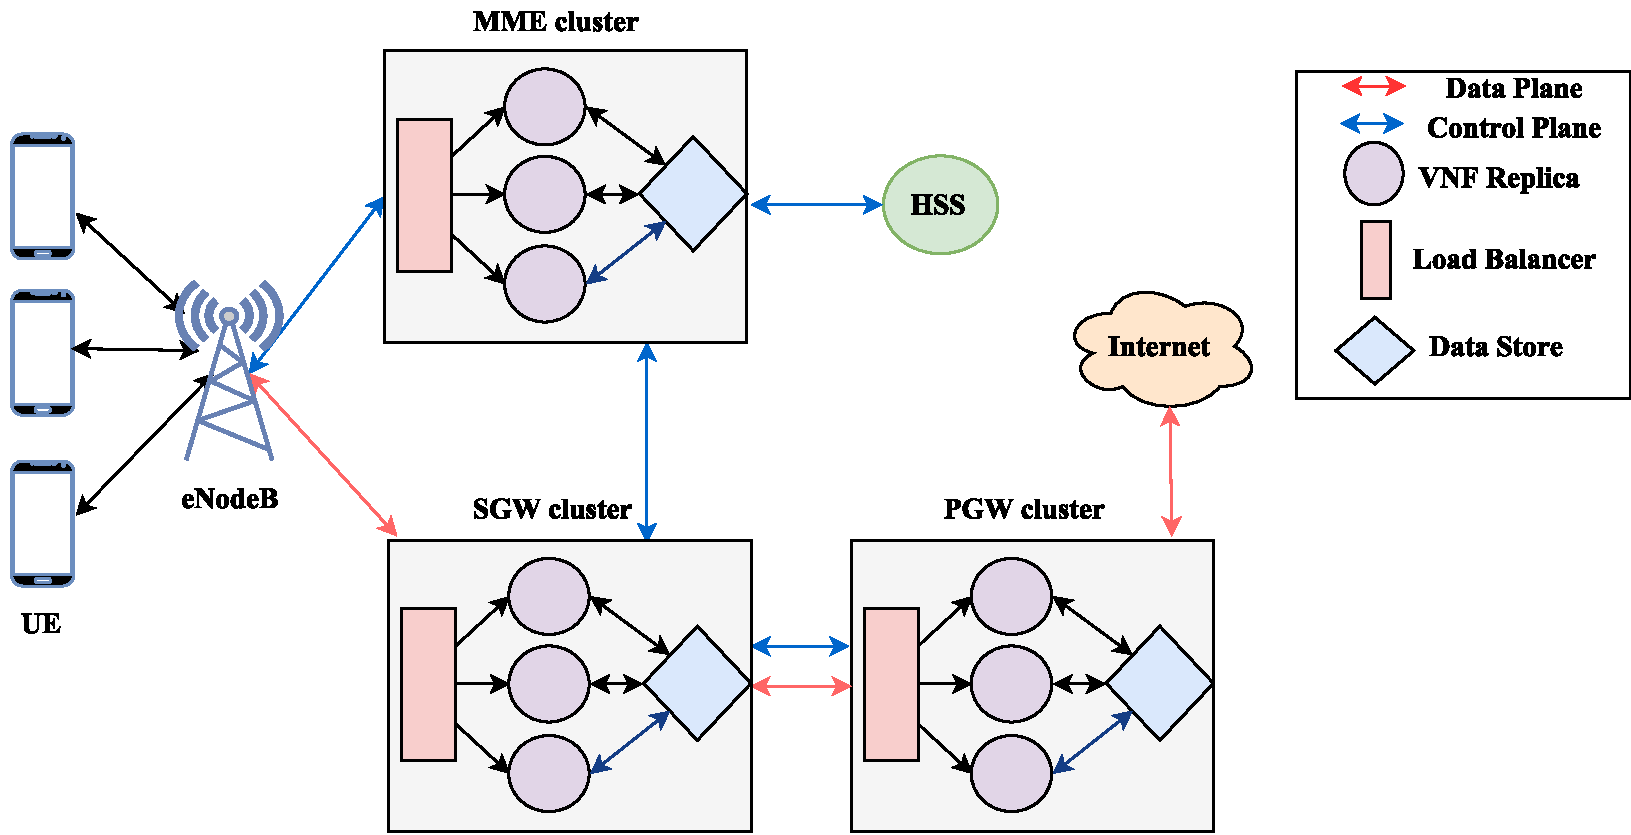
\includegraphics[scale=0.6]{images/depc}
\caption{vEPC Setup.}
\label{setup}

\end{figure}

\item

The VM details of a standard experiment setup of our vEPC is listed in Table \ref{guest}. Specification for MME, SGW and PGW are for a single instance. A two replica system having two MMEs, two SGWs and two PGWs will require each of the instances to have the mentioned specification.
\begin{table}[H]
\centering
\caption{Individual component specification}
\label{guest}
\begin{tabular}{@{}|l|c|l|l|l|@{}}
\toprule
\cellcolor[HTML]{FFFFFF}\textbf{COMPONENT}                                                                                   & \multicolumn{1}{l|}{\textbf{CPU CORES}} & \textbf{RAM} & \textbf{DISK} & \textbf{OS}  \\ \midrule
\cellcolor[HTML]{FFFFFF}RAN, SINK                                                                                           & 8                                       & 8 GB         & 10 GB         & Ubuntu 14.04 \\ \midrule
\cellcolor[HTML]{FFFFFF}MME, SGW, PGW, HSS (per instance)                                                                                  & 1                                       & 2 GB         & 10 GB         & Ubuntu 14.04           \\ \midrule
\cellcolor[HTML]{FFFFFF}\begin{tabular}[c]{@{}l@{}}MME LOAD BALANCERS\\ SGW LOAD BALANCERS\\ PGW LOAD BALANCERS\end{tabular} & 2                                       & 4 GB         & 10 GB         & Ubuntu 14.04 \\ \midrule
LEVELDB CLUSTER                                                                                                              & 8                                       & 8 GB         & 20 GB          & Ubuntu14.04  \\  \bottomrule
\end{tabular}
\end{table}



Before proceeding, ensure proper communication among all VMs through the use of \cf{ping} command. Also, note down the \cf{eth0} IP addresses of VMs for future references.

\item Distribute the source code files into six sets according to the table~\ref{distribution} below. Eact set of \cf{.cpp/.h} files correspond to one of the EPC modules. Note that in table~\ref{distribution}, each file name (e.g., \cf{diameter}) corresponds to both \cf{.cpp} and \cf{.h} files (\cf{diamter.cpp} and \cf{diameter.h}).

\begin{table}[H]

\caption{Setup: Source code distribution.}
\centering
\label{distribution}
\def\arraystretch{1.5}

\begin{tabular}{|c|c|c|c|c|c|c|}

\hline
\textbf{MODULE} & \textbf{MME} & \textbf{HSS} & \textbf{SGW} & \textbf{PGW} & \textbf{RAN} & \textbf{SINK} \\
\hline
diameter & \T & \T & \T & \T & \T & \T \\
gtp & \T & \T & \T & \T & \T & \T \\
hss & & \T & & & & \\
hss\_server & & \T & & & & \\
mme & \T & & & & & \\
mme\_server & \T & & & & & \\
mysql & & \T & & & & \\
network & \T & \T & \T & \T & \T & \T \\
packet & \T & \T & \T & \T & \T & \T \\
pgw & & & & \T & & \\
pgw\_server & & & & \T & & \\
ran & & & & & \T & \\
ran\_simulator & & & & & \T & \\
s1ap & \T & \T & \T & \T & \T & \T \\
sctp\_client & \T & & & & \T & \\
sctp\_server & \T & \T & & & & \\
security & \T & & & & \T & \\
sgw & & & \T & & & \\
sgw\_server & & & \T & & & \\
sink & & & & & & \T \\
sink\_server & & & & & & \T \\
sync & \T & \T & \T & \T & \T & \\
telecom & \T & & & & \T & \\
tun & & & & & \T & \T \\
udp\_client & \T & & \T & \T & \T & \T \\
udp\_server & & & \T & \T & \T & \T \\
utils & \T & \T & \T & \T & \T & \T \\
\hline

\end{tabular}

\end{table}

\item Once source code files are segregated for each module (MME, HSS, SGW, PGW, RAN, SINK), place each set of files in its corresponding VM. Perform the following steps for each VM.

\item Copy the \cf{install.sh} file from \cf{scripts} folder and run it to have all the required packages/tools in all the VMs that will be used for EPC operations. Install any additional tools that might be required (e.g., \cf{gedit, emacs})

\begin{lstlisting}[language=bash]
$ bash install.sh
\end{lstlisting}



\item Open the utils\.h file for the module.
\item Set DEBUG flag to 0/1 according to your need of debug outputs.
\item Set UE\_BINDING flag to 1/2/3 for Always sync/ Session sync/ No sync for the requirement mode of operation in control plane.
\item Set NOCACHE to 1 to enable Always sync mode in data plane and 0 for Session synch mode in data plane.
\item Set RAN as the current IP of the ran simulator system. In case multiple RAN are used set the RAN2 and RAN3 to the IP address of the other RAN VMs (assuming there are 3 parallel RANs).
\item Set MMELB to the ip address of the MME load balancer.
\item Set SGWLB to the ip address of the SGW load balancer.
\item Set PGWLB to the ip address of the PGW load balancer.
\item Set SINK to the ip address of the SINK system. In case multiple SINKs set SINK2 and SINK3 to the IP address of the other SINK VMs.

\begin{itemize}
\item \textbf{Set up RAN Simulator}\\
\textit{Note: Perform the following steps with the ran simulator code module only}
\begin{enumerate}
\item Set DATA\_TRANSFER flag to 0/1 for choice between control plane / data plane operations.
\item Set DSR = 99 for ran simulator as it does not need a data store integration. Refer to in code documentation  in utils.h for more information.
\item compile using the command 
\begin{lstlisting}[language=bash]
$ make ransim.out
\end{lstlisting}
\item run using the command for control plane operation:
\begin{lstlisting}[language=bash]
./mme.out <num of parallel UEs> <Duration of experiments>
\end{lstlisting}
\item run using the command for data plane operation:
\begin{lstlisting}[language=bash]
./ransim.out <num of parallel UEs> <Inpul load generated from each UE>
\end{lstlisting}
\end{enumerate}

\item \textbf{Set up MME}\\

\textit{Note: Perform the following steps with the MME code module only and for each of the parallel MME replicas.}
\begin{enumerate}

\item Open the utils\.h file for the module.
\item set MME1 to the ip address of the current MME system. In case of multiple replicas for the MME cluster, please specify the next replicas IP address ( assuming 2 more parallel replicas) as MME2 and MME3.
\item Set INIT\_VAL TO 1000000 / 4000000 / 7000000 for different replicas to maintain a disjoint range for UE tunnel id assignment.
\item Set REP to 1 to enable synchronization with sibling replicas.
\item Set DSR to 0/1/2/3 for integration services with different data stores. Refer to in code documentation for more details.
\item compile using the command 
\begin{lstlisting}[language=bash]
$ make mme.out
\end{lstlisting}
\item run using the command for control plane operation:
\begin{lstlisting}[language=bash]
./mme.out <num of worker threads for control plane>
\end{lstlisting}

\end{enumerate}

\item \textbf{Set up SGW}\\

\textit{Note: Perform the following steps with the SGW code module only and for each of the parallel SGW replicas.}
\begin{enumerate}

\item Open the utils\.h file for the module.
\item set SGW to the ip address of the current MME system. In case of multiple replicas for the SGW cluster, please specify the next replicas IP address ( assuming 2 more parallel replicas) as SGW2 and SGW3.
\item Set REP to 1 to enable synchronization with sibling replicas.
\item Set DSR to 0/1/2/3 for integration services with different data stores. Refer to in code documentation for more details.
\item compile using the command 
\begin{lstlisting}[language=bash]
$ make sgw.out
\end{lstlisting}
\item run using the command for control plane operation:
\begin{lstlisting}[language=bash]
./sgw.out <threadCount1> <threadCount2> <threadCount3> 

\end{lstlisting}
threadCount\# is worker count for control plane, uplink and downlink data plane

\end{enumerate}
\item \textbf{Set up PGW}\\

\textit{Note: Perform the following steps with the PGW code module only and for each of the parallel PGW replicas.}
\begin{enumerate}

\item Open the utils\.h file for the module.
\item set PGW1 to the ip address of the current PGW system. In case of multiple replicas for the PGW cluster, please specify the next replicas IP address ( assuming 2 more parallel replicas) as PGW2 and PGW3.
\item Set REP to 1 to enable synchronization with sibling replicas.
\item Set DSR to 0/1/2/3 for integration services with different data stores. Refer to in code documentation for more details.
\item compile using the command 
\begin{lstlisting}[language=bash]
$ make pgw.out
\end{lstlisting}
\item run using the command for control plane operation:
\begin{lstlisting}[language=bash]
./pgw.out <threadCount1> <threadCount2> 
\end{lstlisting}
threadCount\# is worker count for control plane/uplink and down link data plane

\end{enumerate}


\item \textbf{Set up HSS}\\

\textit{Note: Perform the following steps with the HSS code module only.}
\begin{enumerate}

\item Open the utils\.h file for the module.
\item set HSS to the ip address of the current HSS system.
\item Set DSR to 0 for integration services with leveldb data store which serves as the hss internal state store for storing user authentication information. Refer to in code documentation for more details.
\item compile using the command 
\begin{lstlisting}[language=bash]
$ make hss.out
\end{lstlisting}
\item run using the command for control plane operation:
\begin{lstlisting}[language=bash]
./hss.out <servingthreadCount> 
\end{lstlisting}
\clearpage
\item {Setting up HSS state store}
\begin{enumerate}

\item Set up a levelDB based key value store \cf{hss} in the VM assigned for HSS.
A levelDB server client implementation is included as part of the release in directory datastore. Any other datastore also can be used as long as it follows identical setup. We describe below the procedure to setup a levelDB datastore. 
\item Copy the setup\_ds directory from the scripts directory.
\item Place the directory in the virtual machine for HSS. 
\item cd to setup\_ds and execute 
\begin{lstlisting}[language=bash]
$ bash install_server.sh
$ bash run_server.sh <ip of the vm>:8090
\end{lstlisting}

\item HSS has a details of authenticated users who can perform attach. To configure data, copy the \textbf{setup\_hss} directory from \textbf{scripts} folder replace the target ip address of levelDB in \textbf{fill\_hss.cpp} and run the following steps to load data. 
\begin{lstlisting}[language=bash]
$ run load_data.sh
\end{lstlisting}
The command should end with a success message if everything worked correctly.
\end{enumerate}

\end{enumerate}
\item \textbf{Set up SINK}\\

\textit{Note: Perform the following steps with the SINK code module only.}
\begin{enumerate}

\item Open the utils\.h file for the module.
\item set SINK to the ip address of the current HSS system.
\item Set DSR to 99 as SINK does not require any data store integration. Refer to in code documentation for more details.
\item compile using the command 
\begin{lstlisting}[language=bash]
$ make sink.out
\end{lstlisting}
\item run using the command for control plane operation:
\begin{lstlisting}[language=bash]
./sink.out <servingthreadCount> 
\end{lstlisting}

\end{enumerate}\end{itemize}

\end{enumerate}
\subsection*{Setup Datastore for MME/ SGW/ PGW}

Refer to instruction provided at LINK.[give link to jash's documentation]


\subsection*{Setup load-balancers}
\label{sds}
The system has been well tested with LVS-DR based load balancer. However, you are free to choose any other layer-4 load-balancer as long as you follow similar configuration. The following section contains configuration of an LVS-DR based load balancer.

Setup three virtual machines for MME/SGW/PGW load balancers as per the specification provided in Table \ref{guest}.


\begin{enumerate}
\item Follow the following steps to setup each of the load-balancers:

\item Edit the ipvsadm configuration as shown below
\begin{lstlisting}[language=bash]
$ vi /etc/default/ipvsadm
# change
AUTO="true"
# change
DAEMON="master"
# change to the interface to use
IFACE="eth0"
\end{lstlisting}
\item Create a new interface with a virtual ip that is different from the ip address of the load balancers. A different IP can serve the purpose of a virtual director to handle a master slave load balancer configuration in case of failure of the load balancer.
\begin{lstlisting}[language=bash]
vi /etc/network/interfaces
# add to the end
auto eth0:0
iface eth0:0 inet static
address <VIP> (VIP that is exposed to clients)
network 10.0.0.0  (your network address)
netmask <subnetmask> (your subnet mask)
root@user:~# ifup eth0:0 
\end{lstlisting}
\item With this procedure the laod balancer network setup is complete. LVS load balancing can be referred from ipvsadm man pages. Load balancing configuration for a certain setup with three replicas is given in the script folder. Next section shows one of the LVS load balancing configuration as an illustration.
[LVS configuration of SGW]
\begin{lstlisting}[language=bash]
ipvsadm -A -u <SGW_VIP>:7000 -s rr
ipvsadm -a -u <SGW_VIP>:7000 -r <Replica 1 IP>:7000 -g -w 1
ipvsadm -a -u <SGW_VIP>:7000 -r <Replica 2 IP>:7000 -g -w 1
ipvsadm -a -u <SGW_VIP>:7000 -r <Replica 3 IP>:7000 -g -w 1

ipvsadm -A -u <SGW_VIP>:7100 -s rr
ipvsadm -a -u <SGW_VIP>:7100 -r <Replica 1 IP>:7100 -g -w 1
ipvsadm -a -u <SGW_VIP>:7100 -r <Replica 2 IP>:7100 -g -w 1
ipvsadm -a -u <SGW_VIP>:7100 -r <Replica 3 IP>:7100 -g -w 1

ipvsadm -A -u <SGW_VIP>:7200 -s rr
ipvsadm -a -u <SGW_VIP>:7200 -r <Replica 1 IP>:7200 -g -w 1
ipvsadm -a -u <SGW_VIP>:7200 -r <Replica 2 IP>:7200 -g -w 1
ipvsadm -a -u <SGW_VIP>:7200 -r <Replica 3 IP>:7200 -g -w 1

\end{lstlisting}
\item The load balancer configuration also requires an iptables entry at the MME/SGW/PGW replicas.
\begin{lstlisting}[language=bash]
iptables -t nat -A PREROUTING -d <SGW_VIP> -j REDIRECT
\end{lstlisting}
More information on LVS setup can be found  \href{https://www.server-world.info/en/note?os=Ubuntu_14.04\&p=lvs}{\color{blue}here}.
\end{enumerate}

\textit{[NOTE: The complete script for all load balancing rules for MME, SGW, PGW and iptables rules scrripts are provided in the script directory for reference.]}

The vEPC setup would be now complete and you can proceed to experimenting with our vEPC using different types of traffic. A sketch of the implemented setup is given in Figure \ref{setup}. Communication among modules will take place according to the blue/red  lines given in Figure \ref{setup}.


\subsection*{Generating Control traffic}

For experiments with control traffic, we simulate a number of concurrent UEs in the RAN simulator and make the UEs continuously perform attach and detach procedures with the EPC, to create a continuous stream of control traffic. We increase or decrease load on the EPC by varying the number of concurrent UE threads loading the EPC. A detailed description of the procedure is given below.

\begin{enumerate}

\item Once the setup is ready, run each vEPC binary executable in its own VM. Usage format of each executable is given in table~\ref{bin_format} below. Please look at the \cf{developer\_manual.pdf} of vEPC 1.0 under \cf{doc} folder to understand more about the command line parameters used with each executable.

\begin{table}[H]

\caption{Usage format of binary executables.}
\centering
\label{bin_format}
\def\arraystretch{1.5}

\begin{tabular}{|c|p{11.5 cm}|}

\hline
\textbf{MODULE} & \textbf{USAGE} \\
\hline
MME & \cf{./mme.out <\#S1-MME threads>} \\
HSS & \cf{./hss.out <\#S6a threads>} \\
SGW & \cf{./sgw.out <\#S11 threads> <\#S1 threads> <\#S5 threads>} \\
PGW & \cf{./pgw.out <\#S5 threads> <\#SGi threads>} \\
\hline

\end{tabular}

\end{table}

A sample run of vEPC modules is given below.
~\\ \textbf{MME:}

\begin{lstlisting}[language=bash]
$ ./mme.out 50 (to be done at each mme instance)\\

\end{lstlisting}
\textbf{HSS:}
\begin{lstlisting}[language=bash]
$ ./hss.out 50 
\end{lstlisting}

\textbf{SGW:}
\begin{lstlisting}[language=bash]
$ ./sgw.out 50 50 50 (to be done at each instance)
\end{lstlisting}
(to be done at each sgw instance)\\
\textbf{PGW:}
\begin{lstlisting}[language=bash]
$ ./pgw.out 50 50 (to be done at each instance)
\end{lstlisting}
\item \textbf{RAN:} Open \cf{ran\_simulator.cpp} and comment out the following code sections.

\begin{itemize}

\item \cf{data\_transfer} section under the \cf{simulate} function.

\item \cf{tun} and \cf{traffic\_monitor} sections under the \cf{run} function.

\end{itemize}

By doing this, you are simulating \cf{RAN} objects that generate only control traffic.

\item \textbf{RAN:} Rerun the \cf{makefile} for the RAN module to make the binary executable for generating only control traffic.

\begin{lstlisting}[language=bash]
$ make ransim.out
\end{lstlisting}

\item \textbf{RAN:} Start RAN simulator with appropriate parameters as given below. This will generate the required amount of control traffic for the given time duration.

\begin{center}

\cf{./ransim.out <\#RAN threads> <Time duration>}

\end{center}

A sample run is as follows.

\begin{lstlisting}[language=bash]
$ ./ransim 10 100
\end{lstlisting}

\end{enumerate}

\noindent \textbf{Fault tolerance experiments:}

For fault tolerant experiments the lvs load balancer needs to be  configured with the keepalived extension. A sample working script for the  MME load balancer is available at the script/LBrules directory.\\


\noindent Enabling the keepalived extension:\\
1. Install keepalived by sudo apt-get install keepalived\\
2. Copy the keepalived script provided at the above mentioned script location.\\
3. Start keepalived in root with command: service keepalived start.\\
4. [optional] For stopping keepalived mode we can use service keepalived stop

Use the ran simulator code provided in the misc directory in the folder structure for fault tolerance operations. This RAN version has all procedure retry codes required. Start EPC in a 3 replica mode with around 30 concurrent UEs. Stop one of the replica by killing its server. The ran will list out number of registration attempts and number of successful attempts. It also informs about number of extra retry count that was required for successful registration compared to a normal case.


\subsection*{Generating Data traffic}

For experiments with data traffic, we attach a specified number of UEs to the EPC from the RAN simulator, and pump traffic from the RAN to the sink. A traffic generating tool called \cf{iperf3} is employed, using which TCP data can be sent with a given bandwidth and time duration. To generate traffic, \cf{iperf3} process is started in Server mode at the Sink module and the corresponding \cf{iperf3} Client process is started at the RAN simulator with the required input data rate and time duration parameters. A detailed description of the procedure is given below.

\begin{enumerate}

\item Begin vEPC modules (MME, HSS, SGW, PGW) as explained before.

\item \textbf{SINK:} Start the Sink module with the required number of \cf{iperf3} servers.

\begin{center}

\cf{./sink.out <\#iperf3 servers>}

\end{center}

A sample run is as follows.

\begin{lstlisting}[language=bash]
$ ./sink 10
\end{lstlisting}

\item \textbf{RAN:} Open \textbf{ran\_simulator\_data.cpp} and rename it to \textbf{ran\_simulator.cpp}. 
\item Open utils.h and set DATA\_TRANSFER to 1 to change ran simulator mode.
\item \textbf{RAN:} Open \cf{ran.cpp} and set the duration of \cf{iperf3} data transfer - \cf{dur} under the \cf{transfer\_data} function. Note that this duration has to be smaller than the overall duration given as command line parameter while running RAN simulator. Input data rate is currently fixed at 1 Mbps. It can be modified as per requirements.

\item \textbf{RAN:} Rerun the \cf{makefile} for the RAN module to reflect the updates in the binary executable.

\begin{lstlisting}[language=bash]
$ make ransim.out
\end{lstlisting}

\item \textbf{RAN:} Now begin the RAN simulator as explained before. This will simulate the required number of \cf{RAN} objects, generating both control traffic and data traffic in sequence, for the given time duration. Note that the number of \cf{RAN} objects created has to be equal or greater than the number of \cf{iperf3} servers started at Sink module.

\end{enumerate}

\subsection*{Performance results}

\paragraph*{Control traffic}

~\\ Two performance metrics would be reported at the end of control traffic experimentation. These parameters are given below. No additional scripts/coding would be required to produce these parameters as they are computed along with the generation of control traffic. 

\begin{enumerate}

\item \textbf{Throughput}, the number of registration requests successfully completed by the EPC per second

\item \textbf{Latency}, the time taken by a registration to complete

\end{enumerate}

\paragraph*{Data traffic}

~\\ While experimenting with data traffic, the following steps need to be followed to obtain performance results.

\begin{enumerate}

\item \textbf{SINK:} Copy the \cf{find\_bw.sh} file from \cf{scripts} folder. Just before starting the RAN simulator, run this script at the Sink module. This will measure the required throughput value. A file named \cf{bw.txt} will be created, which contains the various throughput values (in bytes/second): Uplink, Downlink, Total (Uplink + Downlink). 

\textbf{Format:}
\begin{center}

\cf{bash find\_bw.sh -i <interface> -s <duration> -c <count> -n <\#UEs>} 

\end{center}

\textbf{Sample run:}

\begin{lstlisting}[language=bash]
$ bash find_bw.sh -i eth0 -s 100 -c 1 -n 1
\end{lstlisting}
[Note: find\_bw.sh can be found in the scripts folder]
\item \textbf{RAN:} Before starting the RAN simulator, open \cf{ran\_simulator.cpp} and uncomment the \cf{RTT} code section under the \cf{simulate} function. This will create a \cf{ping.txt} file, which contains the Round Trip Time (RTT) latency values for the data transfer in milliseconds. Note that the time duration under \cf{ping} function need to be set according to the time duration of the user data transfer.

\end{enumerate}

With the procedure explained above, two performance metrics would be obtained at the end of data traffic experimentation. These parameters are given below.

\begin{enumerate}

\item \textbf{Throughput}, the amount of data traffic successfully forwarded by the EPC gateways to the Sink per second

\item \textbf{RTT Latency}, the amount of processing overhead added by the EPC gateways in the data
plane, as measured by a ping command during load test

\end{enumerate}

\section*{Our results}
On a succesful setup of a 3 replica distributed vEPC 2.0 the following throughput results may be observed.\\

\noindent\textbf{Control plane throughput results:}

 \textbf{No sync} mode evaluated with 1, 2 and 3 replicas configuration of MME / SGW / PGW.
The graph captures number of registration/second vs number of concurrent UEs. The saturation throughput for 1, 2, 3 replicas respectively are 4283, 6917, 10215.6 registrations/second.

\textbf{Session-sync} mode evaluated with 1, 2 and 3 replicas configuration of MME / SGW / PGW.
The saturation throughput for 1, 2, 3 replicas respectively are 2016, 3752, 5004 registrations/second.

\textbf{Always-sync} mode evaluated with 1, 2 and 3 replicas configuration of MME / SGW / PGW.
The saturation throughput for 1, 2, 3 replicas respectively are 1249, 2195, 2885 registrations/second.\\

\noindent\textbf{Data plane throughput results:}

\textbf{Session-sync} mode shows EPC data plane scaling in Session sync mode evaluated with 1, 2 and 3 replicas configuration of MME / SGW / PGW. The saturation data plane throughput for 1,2,3 replicas respectively are 233, 405, 504 Mbps.

\textbf{Always-sync} mode shows EPC data plane scaling in Always sync mode evaluated with 1, 2 and 3 replicas configuration of MME / SGW / PGW. The saturation data plane throughput for 1,2,3 replicas respectively are 43, 83, 121 Mbps.\\


\noindent\textbf{Tips to avoid common mistakes in setup:}

\begin{itemize}
\item Check enabling of virtual interfaces at all load balancers while setting up VIP.
\item Check consistency between ip address mentioned in utils.h for all modules and their real ip addresses
\item Check iptables rules set installation in all worker replicas of MME, SGW and PGW.
\item Check correctness the UE INIT\_VALUE range for all MME replicas.
\item Enable ip fowrading in all Load balancers.
\item Check that the load balancers has been set with source\_hash\_ipvs3.conf for No sync mode.
\item Check use of proper DSR setting.
\end{itemize}

\end{document}